\documentclass[tikz,border=8pt]{standalone}
\usetikzlibrary{arrows.meta,positioning}
\begin{document}
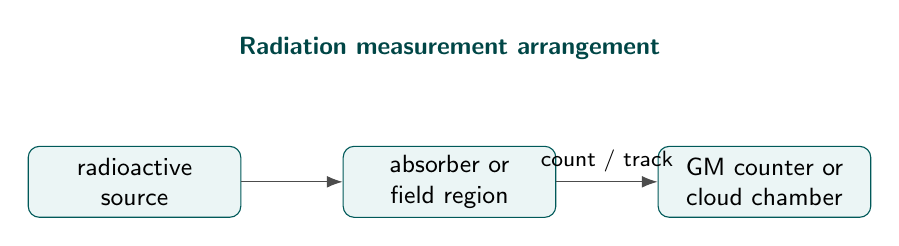
\begin{tikzpicture}[box/.style={draw=teal!70!black,fill=teal!8,rounded corners,minimum width=2.7cm,minimum height=.9cm,align=center,font=\sffamily\small},a/.style={-{Latex[length=2mm]},draw=black!70}]
\node[font=\sffamily\bfseries\small,text=teal!55!black] at (0,1.7) {Radiation measurement arrangement};
\node[box] (s) at (-4,0) {radioactive\\source};
\node[box] (g) at (0,0) {absorber or\\field region};
\node[box] (d) at (4,0) {GM counter or\\cloud chamber};
\draw[a] (s)--(g); \draw[a] (g)--node[above,font=\sffamily\footnotesize]{count / track} (d);
\end{tikzpicture}
\end{document}

